% !TEX root = ../main.tex

\section{Термический ветер и его влияние на изменения ветра с высотой}
\begin{wrapfigure}[15]{R}{0.3\linewidth}
	\vspace{-6ex}
	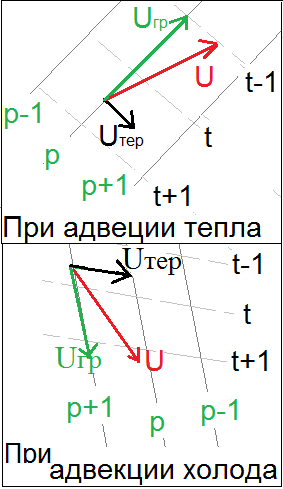
\includegraphics[width=16 mm]{Thermal_wind}
\end{wrapfigure}

\textbf{Термический ветер} - прирост геострофического ветра от одного уровня к др за счет ср гориз-ого градиента T в слое между этими уровнями.\\
Тёплый воздух, стараясь выровнять T, устремляется в сторону более холодного; поток воздуха устойчив тогда, когда будет направлен параллельно изотермам (область холодного слева в С полушарии).\\
При адвекция тепла наблюдается правый поворот ветра (по ч.c), а при адвекция холода - левый поворот.